
\section{\textit{Master-Slave}}\label{appendix:master_slave}

\subsection{Contexto}   

O exemplo a seguir baseia-se na Figura \ref{fig:master_sl_diagrama} apresentada na Seção \ref{sec:master_slave}. Em resumo, um agente \textit{ConcreteCashFlowAgent} deseja obter o balanço total de pagamentos da sua caixa registradora.

\subsection{Preparação do ambiente}\label{subsec:preparacao_ambiente_eclipse}

O exemplo foi rodado em sistema operacional Ubuntu 16.04, utilizando a IDE Eclipse Neon versão 4.6.3. Os seguintes passos devem ser seguidos para rodar este exemplo e os exemplos a seguir:

\begin{enumerate}
    \item Faço o download do código através do GitHub\footnote{https://github.com/tainarareis/MultiagentsSystemsCatalog} e descomprima a pasta;
    \item Abra a IDE Eclipse Neon;
    \item Clique em \textit{File > Import > General > Existing Projects into Workspace};
    \item Selecione a pasta que contém o código;
    \item Clique em \textit{Finish};
    \item No menu \textit{Package Explorer} navegue até a classe \textit{Main} do \textit{package} \textit{\textbf{master_slave}} e clique em \textit{Run}.
\end{enumerate}

\subsection{Classe \textit{Main}}

Basicamente, o \textit{cashFlowAgent}, instância de \textit{ConcreteCashFlowAgent}, precisa ler um arquivo CSV para que, em seguida, obtenha o balanço todos dos pagamentos realizados naquele dia.

\begin{lstlisting}
package master_slave;

public class Main {
	
	public static void main(String[] args) {
		//Read the csv file with the Cash Register
		ConcreteCashFlowAgent cashFlowAgent = new ConcreteCashFlowAgent();
		cashFlowAgent.readCSV();
		
		//Get total balance of payments
		cashFlowAgent.getResult();
	}
}
\end{lstlisting}

\subsection{Classes \textit{MasterAgent} \textit{ConcreteCashFlowAgent}}

A classe \textit{MasterAgent} é interface para que a classe concreta \textit{ConcreteCashFlowAgent} e outras concretas que virem a existir possam se basear.

\begin{lstlisting}
package master_slave;

public interface MasterAgent {

	abstract void readCSV();
	
	abstract void getResult();
}
\end{lstlisting}

O \textit{ConcreteCashFlowAgent} possui uma instância \textit{slave} do \textit{ConcreteSlaveAgent} para realizar tarefas de baixo nível para ele. Os métodos \textit{readCSV()} e \textit{getResult()} têm como objetivo controlar como e quando o \textit{slave} executará tais tarefas.

\begin{lstlisting}
package master_slave;

import java.io.BufferedReader;
import java.io.FileReader;
import java.io.IOException;

public class ConcreteCashFlowAgent {

	ConcreteSlaveAgent slave = new ConcreteSlaveAgent();
	
	protected void readCSV() {
    	//Inform file Path
        String csvFile = "/home/tainara/eclipse-workspace/MultiagentSystemsCatalog/src/master_slave/cash_register.csv";
        
        //Each new line is recognized by empty string
        String line = "";
        
        //Comma is used as separator
        String cvsSplitByComma = ","; 

        try (BufferedReader br = new BufferedReader(new FileReader(csvFile))) {

            while ((line = br.readLine()) != null) {

                
                String[] field = line.split(cvsSplitByComma);
                slave.addPayment(Float.parseFloat(field[1]), 
                					Float.parseFloat(field[2]));
                
                System.out.println("Payment [Item= " + field[0] + 
					" , Quantity= " + field[1] + 
					" , Amount=" + field[2] + "]");
                
            }

        } catch (IOException e) {
            e.printStackTrace();
        }
	}
        
   protected void getResult() {
	   float total = slave.getTotalBalance();	
	   System.out.println("The total balance of payments was $" + total);
   }

}
\end{lstlisting}

\subsection{Classes \textit{SlaveAgent} e \textit{ConcreteSlaveAgent}}

A classe \textit{SlaveAgent} possui os métodos comuns para futuros \textit{slaves} deste contexto. A classe \textit{ConcreteSlaveAgent} implementa tais métodos. Basicamente, o \textit{slave} pode adicionar um pagamento (\textit{addPayment(float quantity, float amount)}) e também obter o balanço final (método \textit{getTotalBalance()}). 

\begin{lstlisting}
package master_slave;

public abstract class SlaveAgent {

	protected abstract void addPayment(float quantity, float amount);

	protected abstract float getTotalBalance();
	
}
\end{lstlisting}
 


\begin{lstlisting}
package master_slave;

public class ConcreteSlaveAgent extends SlaveAgent {

	private float totalBalance;
	
	protected void addPayment(float quantity, float amount) {
		float result = quantity * amount;
		this.totalBalance =+result;
	}

	protected float getTotalBalance() {
		return this.totalBalance;
	}

}
\end{lstlisting}



\subsection{Resultados da execução}


Apenas para exemplificar este contexto e o fluxo de eventos que ocorreria quando executada a implementação apresentada, a Figura \ref{fig:master_sl_console} apresenta a saída no console da IDE Eclipse Neon.

\begin{figure}[!h]
\centering
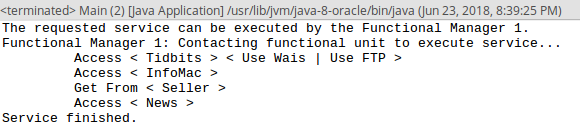
\includegraphics[scale=0.7]{figuras/macron/macron_console.png}
\caption{Saídas do console: \textit{Master-Slave} executa o serviço solicitado.}
\label{fig:master_sl_console}
\end{figure}